\documentclass[11pt,a4paper]{article}

\usepackage[T1]{fontenc}
\usepackage[utf8]{inputenc}
\usepackage{lmodern}
\usepackage{mathptmx}
\usepackage[Symbol]{upgreek}      % upright Greek letters, in the same Times style as the text
\usepackage[margin=2.1cm]{geometry}
\usepackage{microtype}
\usepackage{amsmath,amssymb}
\usepackage{booktabs}
\usepackage{graphicx}
\usepackage[font=small,labelfont=bf,skip=4pt]{caption}
\usepackage{tikz}
\usetikzlibrary{arrows.meta,positioning,calc,decorations.pathreplacing}
\usepackage{enumitem}
\usepackage[numbers,sort&compress]{natbib}
\usepackage[hidelinks]{hyperref}   % plain black text, no coloured links
\usepackage[capitalise,noabbrev]{cleveref}

\setlist{nosep,leftmargin=1.3em}
\setlength{\parskip}{0.3em}
\renewcommand{\topfraction}{0.9}
\renewcommand{\textfraction}{0.07}
\renewcommand{\floatpagefraction}{0.8}

% Every number below is generated from the result files, never typed by hand.
% Auto-generated by make_paper_assets.py -- do not edit by hand.
\newcommand{\bestLeakDeadPct}{96}
\newcommand{\bestLeakLambda}{10}
\newcommand{\bestLeakMode}{mean}
\newcommand{\bestLeakRouting}{0.0003}
\newcommand{\bestLeakValue}{0.0020}
\newcommand{\bestRoutAlivePct}{83}
\newcommand{\bestRoutLeak}{0.296}
\newcommand{\bestRoutValue}{0.40}
\newcommand{\blockOffPositive}{4}
\newcommand{\blockPositive}{19}
\newcommand{\blockRuns}{5}
\newcommand{\blockSig}{10}
\newcommand{\blockSigHolm}{1}
\newcommand{\blockSigTauFifty}{1}
\newcommand{\blockSigTauFive}{3}
\newcommand{\blockSigTauTen}{4}
\newcommand{\blockSigTauTwenty}{2}
\newcommand{\blockSignP}{2.0\times10^{-5}}
\newcommand{\blockTotal}{20}
\newcommand{\budget}{10}
\newcommand{\cgGptSent}{+0.109}
\newcommand{\cgGptTox}{+0.133}
\newcommand{\cgPGptSent}{$<$0.001}
\newcommand{\cgPGptTox}{0.879}
\newcommand{\cgPQwenSent}{0.004}
\newcommand{\cgPQwenTox}{0.007}
\newcommand{\cgQwenSent}{+0.277}
\newcommand{\cgQwenTox}{+0.127}
\newcommand{\contrastFVUlamOne}{0.250}
\newcommand{\contrastFVUlamTen}{1.03}
\newcommand{\contrastRoutLamOne}{0.36}
\newcommand{\degenCorrMax}{-0.28}
\newcommand{\dimGptSent}{+0.404}
\newcommand{\dimGptTox}{+0.130}
\newcommand{\dimQwenSent}{+0.413}
\newcommand{\dimQwenTox}{+0.044}
\newcommand{\dimSentSAEbetter}{0}
\newcommand{\dimSentSAEworse}{12}
\newcommand{\dimSentTotal}{12}
\newcommand{\dimToxSAEbetter}{3}
\newcommand{\dimToxSAEworse}{0}
\newcommand{\dimToxTotal}{8}
\newcommand{\dissBUnw}{-0.447}
\newcommand{\dissBWan}{+0.184}
\newcommand{\dissGUnw}{+0.183}
\newcommand{\dissGWan}{-0.411}
\newcommand{\dissRUnw}{-0.039}
\newcommand{\dissRWan}{+0.001}
\newcommand{\evVanGPT}{80}
\newcommand{\evVanQwen}{96}
\newcommand{\fvuCGGPT}{0.277}
\newcommand{\fvuCGQwen}{0.066}
\newcommand{\fvuVanGPT}{0.203}
\newcommand{\fvuVanQwen}{0.045}
\newcommand{\layerDisagree}{4}
\newcommand{\layerFracMax}{85}
\newcommand{\layerFracMin}{27}
\newcommand{\layerGptAUC}{0.816}
\newcommand{\layerGptLoss}{45}
\newcommand{\layerGptProbe}{11}
\newcommand{\layerGptSteer}{7}
\newcommand{\layerScans}{4}
\newcommand{\leakRatioBestVsRout}{146}
\newcommand{\leakRoutingCorr}{+0.03}
\newcommand{\nPrimaryRuns}{5}
\newcommand{\nRuns}{6}
\newcommand{\nSynthSeeds}{20}
\newcommand{\penformConfigs}{12}
\newcommand{\penformSeeds}{2}
\newcommand{\qtoxLfifteenEff}{+0.062}
\newcommand{\qtoxLfifteenPPL}{37.6}
\newcommand{\qtoxLtenEff}{+0.056}
\newcommand{\qtoxLtenPPL}{6.5}
\newcommand{\scarGptSent}{+0.118}
\newcommand{\scarGptTox}{+0.194}
\newcommand{\scarPGptSent}{$<$0.001}
\newcommand{\scarPGptTox}{0.022}
\newcommand{\scarPQwenSent}{$<$0.001}
\newcommand{\scarPQwenTox}{0.075}
\newcommand{\scarQwenSent}{+0.147}
\newcommand{\scarQwenTox}{+0.075}
\newcommand{\specMax}{16.6}
\newcommand{\specMaxBuf}{4.33}
\newcommand{\specMaxLamFive}{14.0}
\newcommand{\specNoBufLamFive}{0.91}
\newcommand{\specNoBufLamOne}{1.5}
\newcommand{\specOffMax}{1.65}
\newcommand{\specOffMin}{0.99}
\newcommand{\sqFVUspread}{1.2\times10^{-4}}
\newcommand{\sqLeakLamThirty}{0.435}
\newcommand{\sqLeakLamZero}{0.495}
\newcommand{\sqPenShare}{0.5}
\newcommand{\sqPenTermThirty}{8.7\times10^{-4}}
\newcommand{\sqRoutMax}{0.012}
\newcommand{\synthBAliveMin}{100}
\newcommand{\synthRouting}{0.35}
\newcommand{\synthRoutingOff}{0.010}
\newcommand{\vanFVUpenform}{0.173}
\newcommand{\vsSSVgptPmax}{0.40}
\newcommand{\vsSSVgptPmin}{0.24}
\newcommand{\vsSSVgptPositive}{3}
\newcommand{\vsSSVgptSig}{0}
\newcommand{\vsSSVgptTotal}{4}
\newcommand{\vsSSVqwenPositive}{8}
\newcommand{\vsSSVqwenPrimSig}{4}
\newcommand{\vsSSVqwenPrimTotal}{6}
\newcommand{\vsSSVqwenSig}{6}
\newcommand{\vsSSVqwenSigHolm}{3}
\newcommand{\vsSSVqwenTotal}{8}
\newcommand{\vsScarQwenSig}{1}
\newcommand{\vsScarSig}{1}
\newcommand{\vsScarTotal}{12}

% Auto-generated by make_ea_assets.py -- do not edit by hand.
\newcommand{\ghBadGen}{+0.111}
\newcommand{\ghBadNeg}{+30.1}
\newcommand{\ghBadNegHi}{+31.7}
\newcommand{\ghBadNegLo}{+28.4}
\newcommand{\ghBadPos}{+9.1}
\newcommand{\ghGoodGen}{+0.092}
\newcommand{\ghGoodNeg}{+6.7}
\newcommand{\ghGoodNegHi}{+7.2}
\newcommand{\ghGoodNegLo}{+6.5}
\newcommand{\ghGoodPos}{+26.6}
\newcommand{\ghRandGen}{+0.078}
\newcommand{\ghRandNeg}{+9.7}
\newcommand{\ghRandNegHi}{+14.6}
\newcommand{\ghRandNegLo}{+6.6}
\newcommand{\ghRandPos}{+11.1}
\newcommand{\ghRelearnBad}{0.54}
\newcommand{\ghRelearnRand}{0.52}
\newcommand{\ghRouting}{0.37}
\newcommand{\ghSeeds}{3}
\newcommand{\ghWikiBucket}{120}
\newcommand{\ghWikiCostPct}{105}
\newcommand{\ghWikiPlain}{59}
\newcommand{\glBadGen}{-0.028}
\newcommand{\glBadNeg}{+9.0}
\newcommand{\glBadNegHi}{+9.0}
\newcommand{\glBadNegLo}{+9.0}
\newcommand{\glBadPos}{+8.6}
\newcommand{\glGoodGen}{-0.055}
\newcommand{\glGoodNeg}{+8.3}
\newcommand{\glGoodNegHi}{+8.3}
\newcommand{\glGoodNegLo}{+8.2}
\newcommand{\glGoodPos}{+8.1}
\newcommand{\glRandGen}{+0.022}
\newcommand{\glRandNeg}{+9.3}
\newcommand{\glRandNegHi}{+10.6}
\newcommand{\glRandNegLo}{+8.0}
\newcommand{\glRandPos}{+9.1}
\newcommand{\glRelearnBad}{0.67}
\newcommand{\glRelearnRand}{0.68}
\newcommand{\glRouting}{0.00}
\newcommand{\glSeeds}{3}
\newcommand{\glWikiBucket}{59}
\newcommand{\glWikiPlain}{59}
\newcommand{\gtBadGen}{+0.048}
\newcommand{\gtBadNeg}{+26.5}
\newcommand{\gtBadNegHi}{+29.2}
\newcommand{\gtBadNegLo}{+24.8}
\newcommand{\gtBadPos}{+9.6}
\newcommand{\gtGoodGen}{+0.080}
\newcommand{\gtGoodNeg}{+7.7}
\newcommand{\gtGoodNegHi}{+7.9}
\newcommand{\gtGoodNegLo}{+7.6}
\newcommand{\gtGoodPos}{+21.6}
\newcommand{\gtRandGen}{+0.085}
\newcommand{\gtRandNeg}{+10.5}
\newcommand{\gtRandNegHi}{+13.0}
\newcommand{\gtRandNegLo}{+7.5}
\newcommand{\gtRandPos}{+12.2}
\newcommand{\gtRelearnBad}{0.63}
\newcommand{\gtRelearnRand}{0.63}
\newcommand{\gtRouting}{0.29}
\newcommand{\gtSeeds}{3}
\newcommand{\gtWikiBucket}{69}
\newcommand{\gtWikiCostPct}{19}
\newcommand{\gtWikiPlain}{58}
\newcommand{\slBadGen}{-0.011}
\newcommand{\slBadNeg}{+19.7}
\newcommand{\slBadNegHi}{+21.2}
\newcommand{\slBadNegLo}{+18.3}
\newcommand{\slBadPos}{+7.3}
\newcommand{\slGoodGen}{-0.040}
\newcommand{\slGoodNeg}{+6.9}
\newcommand{\slGoodNegHi}{+9.2}
\newcommand{\slGoodNegLo}{+4.5}
\newcommand{\slGoodPos}{+26.3}
\newcommand{\slRandGen}{+0.001}
\newcommand{\slRandNeg}{+0.2}
\newcommand{\slRandNegHi}{+0.3}
\newcommand{\slRandNegLo}{+0.1}
\newcommand{\slRandPos}{+0.1}
\newcommand{\slRelearnBad}{0.74}
\newcommand{\slRelearnRand}{0.74}
\newcommand{\slRouting}{0.87}
\newcommand{\slSeeds}{2}
\newcommand{\slWikiBucket}{1932}
\newcommand{\slWikiPlain}{1957}
\newcommand{\ssBadGen}{-0.116}
\newcommand{\ssBadNeg}{+3.9}
\newcommand{\ssBadNegHi}{+4.6}
\newcommand{\ssBadNegLo}{+3.2}
\newcommand{\ssBadPos}{-0.4}
\newcommand{\ssGoodGen}{+0.064}
\newcommand{\ssGoodNeg}{-0.3}
\newcommand{\ssGoodNegHi}{+0.1}
\newcommand{\ssGoodNegLo}{-0.8}
\newcommand{\ssGoodPos}{+3.4}
\newcommand{\ssRandGen}{-0.020}
\newcommand{\ssRandNeg}{+0.5}
\newcommand{\ssRandNegHi}{+0.5}
\newcommand{\ssRandNegLo}{+0.4}
\newcommand{\ssRandPos}{+0.4}
\newcommand{\ssRelearnBad}{0.67}
\newcommand{\ssRelearnRand}{0.62}
\newcommand{\ssRouting}{0.92}
\newcommand{\ssSeeds}{2}
\newcommand{\ssWikiBucket}{7208}
\newcommand{\ssWikiPlain}{12579}


% Plain, upright notation.
\newcommand{\z}{\mathbf{z}}
\newcommand{\x}{\mathbf{x}}
\newcommand{\h}{\mathbf{h}}
\newcommand{\Wb}{\mathrm{W}}      % wanted bucket
\newcommand{\Nb}{\mathrm{N}}      % neutral buffer
\newcommand{\Ub}{\mathrm{U}}      % unwanted bucket
\newcommand{\ntag}{n_{\mathrm{tag}}}
\newcommand{\avg}{\operatorname{mean}}

\title{\vspace{-1.6em}\textbf{Reserving Space for Unwanted Behaviour\\ Inside Language Models\\[2pt]
\large Wanted and Unwanted Buckets with a Neutral Buffer}}
\author{K.\ Hima Bindu, Varanasi Sathveek, Vanamala Aravind, Pula Naga Manikanta\\[2pt]
\small Department of Computer Science \& Engineering, National Institute of Technology Andhra Pradesh, India}
\date{\small Extended abstract \,\textbullet\, CARE 2026, Track: Foundations of AI}

\begin{document}
\maketitle
\vspace{-1.2em}

\begin{abstract}
\noindent
A language model stores far more concepts than it has neurons, so the concepts overlap, and
turning one behaviour off usually damages others. We ask a simple question: what if we decide,
\emph{before training}, where an unwanted behaviour is allowed to live? We split a group of units
into a \emph{wanted} bucket, an \emph{unwanted} bucket and a neutral buffer between them, train with
a penalty that sends each kind of input to its own bucket, and afterwards delete the unwanted bucket.
We first test the idea on a small toy network, where deleting the unwanted bucket is up to
\specMax$\times$ more targeted than deleting a random bucket of the same size, but only when the
buffer is present. We then scale it to language models. Inside GPT-2's own neurons, deleting the
unwanted bucket raises perplexity on negative reviews by \gtBadNeg\% but on positive reviews by only
\gtBadPos\%, in all \gtSeeds{} runs, and deleting the wanted bucket does the opposite. For models that
cannot be retrained, we place the same buckets in a sparse autoencoder, where removing the unwanted
bucket beats removing a random one in \blockPositive{} of \blockTotal{} settings. The buckets reliably
capture the unwanted knowledge; reliably changing what the model writes is still an open problem.
\end{abstract}

% ===========================================================================
\section{Background}

Language models do not keep one concept per neuron. They need to represent many more concepts than
they have dimensions, so they store them in overlapping directions, which is known as
\emph{superposition}~\citep{elhage2022toy}. Roughly, a hidden state $\h$ is a sum of concept directions,
\begin{equation}
  \h \;\approx\; \textstyle\sum_{i=1}^{n} f_i\,\mathbf v_i ,
\end{equation}
where $f_i$ says whether concept $i$ is present and $\mathbf v_i$ is its direction. Because these
directions overlap, removing one concept disturbs others. That is why taking out a single behaviour,
such as negative sentiment or toxicity, cleanly is difficult.

Two families of methods try to help. Sparse autoencoders (SAEs) rewrite a model's activations in a
much larger and sparser space, so that each unit is closer to one concept~\citep{bricken2023monosemanticity,cunningham2024sparse,gao2024scaling}.
Activation steering nudges the model while it runs by adding or subtracting a concept
direction~\citep{turner2023actadd,rimsky2024caa}. Neither decides \emph{in advance} where a concept
should be stored.

Our idea is to make that decision before training: reserve a fixed set of units for the unwanted
behaviour, train the model so that the behaviour ends up there, and then delete those units. We first
used a small toy network to state the idea precisely and check that it works at all. In this work we
scale it up: into the neurons of real language models, and into SAEs for models that cannot be
retrained.

% ===========================================================================
\section{Problem and objective}

Three observations shaped the objective.

\textbf{(1) Existing methods do not decide where a concept lives.} Supervised SAEs either tie a
concept to a single unit, as in SCAR~\citep{harle2024scar}, or look for the relevant units after
training, as in SAE-SSV~\citep{he2025saessv}. Neither asks \emph{how many} units a concept should get,
or where features shared by the wanted and unwanted behaviour should go.

\textbf{(2) The obvious training penalty does not work.} A natural penalty is to punish each bucket
for firing on the wrong kind of input. On a properly sparse SAE this barely moves anything: the
separation score went only from \sqLeakLamZero{} to \sqLeakLamThirty{} (0.5 means no separation),
even at thirty times the penalty weight. Worse, a penalty that only says ``do not fire on the wrong
input'' can be satisfied by switching the bucket off entirely.

\textbf{(3) The usual measure cannot tell success from failure.} Such partitions are normally judged by
\emph{leakage}, how much a bucket fires on the wrong input. Across twelve settings we found leakage to
be unrelated to whether the bucket actually carries the concept (correlation $r=\leakRoutingCorr$),
and the best leakage score came from a bucket that was \bestLeakDeadPct\% inactive.

\textbf{Objective.} To reserve, before training, a fixed place for an unwanted behaviour, so that it
can later be removed \emph{by address} rather than by searching for it, and to understand what makes
this work.

% ===========================================================================
\section{Proposed method}

\textbf{Buckets.} Take $m$ units, either MLP neurons of the language model or units of an SAE. With a
tag fraction $\uptau$ and $\ntag=\lfloor\uptau m\rfloor$, we fix three groups before training:
\begin{equation}
  \Wb=\{1,\dots,\ntag\},\qquad
  \Nb=\{\ntag+1,\dots,m-\ntag\},\qquad
  \Ub=\{m-\ntag+1,\dots,m\},
\end{equation}
the wanted bucket, a neutral buffer that is never penalised, and the unwanted bucket
(\cref{fig:method}). The buffer is the new part. Some features are genuinely shared by both kinds of
input, and the buffer gives them somewhere to go instead of forcing them into one bucket.

\textbf{Routing penalty.} For non-negative activations $\z$, let $s_S(\z)=\sum_{j\in S}z_j\big/\sum_j z_j$
be the share of total activity that falls in bucket $S$. Each training token carries the label of the
text it comes from ($y=0$ unwanted, $y=1$ wanted). We use
\begin{equation}
  P=-\tfrac12\Big[\big(\avg_{y=0}s_{\Ub}-\avg_{y=1}s_{\Ub}\big)+\big(\avg_{y=1}s_{\Wb}-\avg_{y=0}s_{\Wb}\big)\Big].
  \label{eq:penalty}
\end{equation}
This rewards the unwanted bucket for \emph{carrying} unwanted activity, not just for staying quiet on
wanted inputs. An empty bucket scores $0$ and perfect routing scores $-1$, so switching the bucket off
no longer pays. The labels are used only inside this training loss. They are never given to the
model as input and are not needed when the model is used. The total loss is
\begin{equation}
  L_{\mathrm{total}}=L_{\mathrm{task}}+\uplambda\,P ,
\end{equation}
where $L_{\mathrm{task}}$ is the normal language-modelling loss when the buckets are inside the model,
or the SAE's reconstruction error when they are inside an SAE, and $\uplambda$ sets the strength of the
penalty. We check that routing actually happened with
$R=\avg_{y=0}s_{\Ub}-\avg_{y=1}s_{\Ub}$, which is $0$ for an empty bucket.

\textbf{Removal.} Inside the model we delete the unwanted neurons outright by zeroing their incoming
and outgoing weights: $W_{\mathrm{in}}[:,\Ub]=0$, $b_{\mathrm{in}}[\Ub]=0$ and $W_{\mathrm{out}}[\Ub,:]=0$.
With an SAE on a frozen model we scale the unwanted units by $(1-\upalpha)$ and add only the resulting
change back to the model,
\begin{equation}
  \h'=\h+\upsigma\big(\mathrm{dec}(\z')-\mathrm{dec}(\z)\big),\qquad \z'_{\Ub}=(1-\upalpha)\,\z_{\Ub},
\end{equation}
where $\upsigma$ undoes the input scaling. Adding only the change keeps the SAE's own reconstruction
error out of the model.

\begin{figure}[t]
\centering
\resizebox{0.92\linewidth}{!}{%
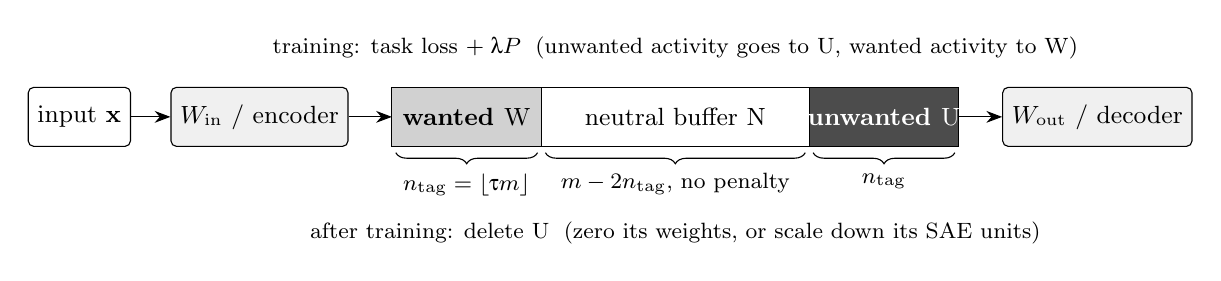
\begin{tikzpicture}[font=\small, >={Stealth[length=2mm]},
  box/.style={draw=black, rounded corners=2pt, minimum height=0.75cm, align=center, fill=white},
  op/.style={draw=black, rounded corners=2pt, minimum height=0.75cm, minimum width=1.5cm, align=center, fill=black!6}]
  \node[box, minimum width=1.2cm] (h) at (0,0) {input $\x$};
  \node[op, right=0.5cm of h] (enc) {$W_{\mathrm{in}}$ / encoder};
  \coordinate (z0) at ($(enc.east)+(0.55,-0.375)$);
  \fill[black!18] (z0) rectangle ++(1.9,0.75);
  \fill[white]    ($(z0)+(1.9,0)$) rectangle ++(3.4,0.75);
  \fill[black!70] ($(z0)+(5.3,0)$) rectangle ++(1.9,0.75);
  \draw[black] (z0) rectangle ++(7.2,0.75);
  \draw[black] ($(z0)+(1.9,0)$) -- ++(0,0.75);
  \draw[black] ($(z0)+(5.3,0)$) -- ++(0,0.75);
  \node[font=\small\bfseries] at ($(z0)+(0.95,0.375)$) {wanted $\Wb$};
  \node at ($(z0)+(3.6,0.375)$) {neutral buffer $\Nb$};
  \node[white, font=\small\bfseries] at ($(z0)+(6.25,0.375)$) {unwanted $\Ub$};
  \draw[decorate,decoration={brace,amplitude=4pt,mirror}] ($(z0)+(0.05,-0.08)$) -- ++(1.8,0)
     node[midway,below=4pt,font=\footnotesize]{$\ntag=\lfloor\uptau m\rfloor$};
  \draw[decorate,decoration={brace,amplitude=4pt,mirror}] ($(z0)+(1.95,-0.08)$) -- ++(3.3,0)
     node[midway,below=4pt,font=\footnotesize]{$m-2\ntag$, no penalty};
  \draw[decorate,decoration={brace,amplitude=4pt,mirror}] ($(z0)+(5.35,-0.08)$) -- ++(1.8,0)
     node[midway,below=4pt,font=\footnotesize]{$\ntag$};
  \node[op, right=0.55cm of {$(z0)+(7.2,0.375)$}] (dec) {$W_{\mathrm{out}}$ / decoder};
  \draw[->] (h) -- (enc);
  \draw[->] (enc.east) -- ($(z0)+(0,0.375)$);
  \draw[->] ($(z0)+(7.2,0.375)$) -- (dec);
  \node[font=\footnotesize] at ($(z0)+(3.6,1.25)$)
     {training: task loss $+\;\uplambda P$ \;(unwanted activity goes to $\Ub$, wanted activity to $\Wb$)};
  \node[font=\footnotesize] at ($(z0)+(3.6,-1.1)$)
     {after training: delete $\Ub$ \;(zero its weights, or scale down its SAE units)};
\end{tikzpicture}}
\caption{\textbf{The bucket idea.} Units are split into a wanted bucket, a neutral buffer and an
unwanted bucket before training. The penalty sends each kind of input to its own bucket, and
afterwards the unwanted bucket is removed by address. The same layout is used inside the model's MLP
layers and inside an SAE.}
\label{fig:method}
\end{figure}

% ===========================================================================
\section{Experiments}

\textbf{Three settings.} (i) \emph{Toy network}: a small classifier ($64\!\to\!32\!\to\!2$) on two
overlapping Gaussian classes, where everything is under our control; \nSynthSeeds{} runs.
(ii) \emph{Buckets inside a language model}: GPT-2~\citep{radford2019gpt2} fine-tuned with buckets in
the MLP neurons of layers 5--9 ($\uptau=0.1$, that is 307 wanted, 2{,}458 neutral and 307 unwanted
neurons per layer), and two GPT-style models (6 and 8 layers) trained \emph{from scratch} with
buckets. (iii) \emph{Buckets inside an SAE} on frozen GPT-2 and Qwen2.5-1.5B~\citep{qwen2024qwen25},
for models that cannot be retrained.

\textbf{Data.} IMDB movie reviews~\citep{maas2011imdb}, with negative sentiment as the unwanted
behaviour, and RealToxicityPrompts~\citep{gehman2020rtp} for toxicity. General writing ability is
checked on WikiText-103~\citep{merity2017wikitext}, which has nothing to do with either behaviour.

\textbf{What we measure.} After deleting a bucket we check (a) \emph{knowledge}: perplexity on
held-out negative versus positive reviews; (b) \emph{behaviour}: how negative the model's
continuations of negative-review openings are, scored by a sentiment classifier; (c) \emph{general
ability}: WikiText perplexity; and (d) \emph{relearning}: how quickly the behaviour returns after
brief retraining. Every deletion is compared with deleting the wanted bucket and with deleting a
\emph{random bucket of the same size}. If the unwanted bucket is no more special than a random one,
the idea has failed.

\textbf{Baselines and fairness.} In the SAE setting we compare with a normal SAE whose units are found
after training (SAE-SSV style), with a single conditioned unit (SCAR style), and with
difference-in-means steering~\citep{rimsky2024caa,arditi2024refusal}. All SAE methods use exactly the
same sparsity and the same number of edited units, and are compared at the same cost in fluency
(a 10\% rise in perplexity), so no method can win just by doing less. We use between 2 and 20 runs per
setting with paired statistical tests. All experiments ran on Kaggle GPUs (NVIDIA P100 and T4).

% ===========================================================================
\section{Results}

\textbf{Toy network: the buffer is what makes it work.} In the toy network (\cref{fig:toy}) we
measure \emph{specificity}, the damage from deleting the unwanted bucket divided by the damage from
deleting a random bucket of the same size. It reaches \specMax$\times$ with a wide buffer and falls to
\specNoBufLamFive, no better than random, when the buffer is removed. Without the penalty it stays
near 1 everywhere. Deleting the unwanted bucket changes accuracy on the unwanted class by $\dissBUnw$
and on the wanted class by $\dissBWan$; deleting the wanted bucket gives the mirror image.

\begin{figure}[t]
  \centering
  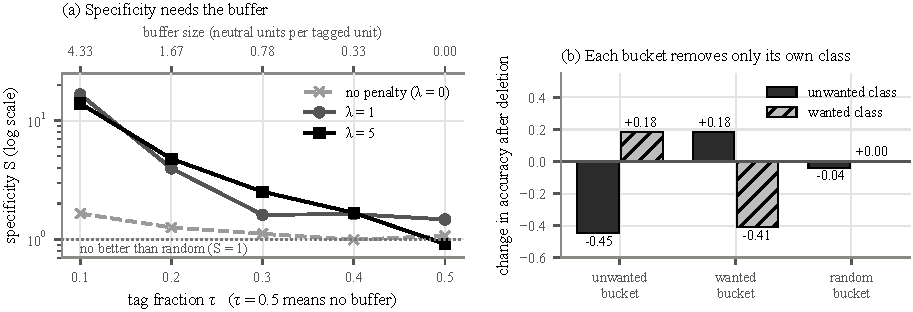
\includegraphics[width=0.94\linewidth]{figures/fig_toy.pdf}
  \caption{\textbf{Toy network, \nSynthSeeds{} runs.} (a) Deleting the unwanted bucket is far more
  targeted than deleting a random bucket, but only when there is a neutral buffer. (b) Each bucket
  removes only its own class; a random bucket removes neither.}
  \label{fig:toy}
\end{figure}

\textbf{Language models: the unwanted bucket holds the unwanted knowledge.} \Cref{fig:inmodel} shows
how perplexity changes after each deletion. With a weak penalty ($\uplambda=1$) no buckets form in
GPT-2 (routing \glRouting), and every deletion looks the same. With $\uplambda=3$, deleting the
unwanted bucket raises perplexity on negative reviews by \gtBadNeg\% (between \gtBadNegLo\% and
\gtBadNegHi\% across runs) but on positive reviews by only \gtBadPos\%. Deleting the wanted bucket
does the reverse (\gtGoodNeg\% against \gtGoodPos\%), and a random bucket hurts both about equally
(\gtRandNeg\% and \gtRandPos\%). This holds in all \gtSeeds{} runs, and costs \gtWikiCostPct\% in
general fluency, far less than the \ghWikiCostPct\% cost at $\uplambda=10$. The models trained from
scratch show the same pattern with routing close to 0.9. In the larger one, deleting the unwanted
bucket costs \slBadNeg\% on negative and \slBadPos\% on positive reviews, while a random bucket costs
almost nothing (\slRandNeg\%).

\begin{figure}[t]
  \centering
  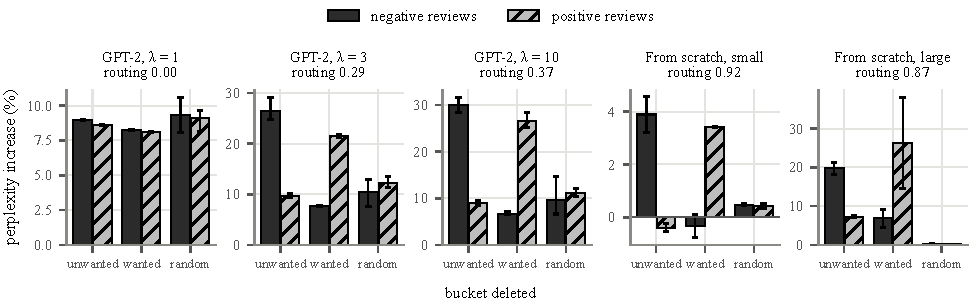
\includegraphics[width=\linewidth]{figures/fig_inmodel.pdf}
  \caption{\textbf{Buckets inside the language model.} Rise in perplexity on held-out negative and
  positive reviews after deleting the unwanted, wanted or a random bucket (mean and range over runs).
  Once buckets form, deleting the unwanted one mainly damages knowledge of negative reviews.}
  \label{fig:inmodel}
\end{figure}

\textbf{SAEs on frozen models: the same holds.} Removing the reserved bucket reduces the behaviour
more than removing a random bucket of the same size in \blockPositive{} of \blockTotal{} settings
(sign test $p=\blockSignP$), across GPT-2 and Qwen and across sentiment and toxicity. \Cref{tab:sae}
compares it with the baselines.

\begin{table}[t]
  \centering\small
  \caption{\textbf{Summary of the SAE experiments} (methods compared at the same fluency cost).}
  \label{tab:sae}
  \begin{tabular}{@{}p{0.50\linewidth}p{0.42\linewidth}@{}}
  \toprule
  Question & Result \\
  \midrule
  Does the reserved bucket beat a random bucket? & Yes, in \blockPositive{} of \blockTotal{} settings \\
  Is a bucketed SAE better than a normal SAE? & On Qwen in \vsSSVqwenSig{} of \vsSSVqwenTotal{} tests; on GPT-2 in \vsSSVgptSig{} of \vsSSVgptTotal{} \\
  Does it beat difference-in-means steering? & Sentiment: no (worse in \dimSentSAEworse{} of \dimSentTotal); toxicity: better in \dimToxSAEbetter{} of \dimToxTotal, never worse \\
  Is leakage a reliable measure? & No, its correlation with routing is $r=\leakRoutingCorr$ \\
  Is the easiest layer to read the best layer to edit? & No, in \layerDisagree{} of \layerScans{} layer scans \\
  \bottomrule
  \end{tabular}
\end{table}

\textbf{What did not work.} Deleting the unwanted bucket did not reliably make the model \emph{write}
less negatively. It did in the small model trained from scratch ($\ssBadGen$ on a 0--1 negativity
score) but not in the larger one ($\slBadGen$) or in GPT-2 ($\gtBadGen$). The knowledge also comes
back after brief retraining about as fast as after a random deletion (\gtRelearnBad{} against
\gtRelearnRand{} in GPT-2). We also found that the layer where a concept is easiest to read with a
simple probe is never the best layer to edit; on GPT-2, choosing it loses \layerGptLoss\% of the
possible effect.

% ===========================================================================
\section{What we infer}

\begin{itemize}
  \item \textbf{It is possible to decide in advance where a behaviour lives.} With the routing
        penalty, the unwanted knowledge really does end up in the reserved bucket, both inside the
        model's own neurons and inside an SAE, and deleting the bucket removes that knowledge
        selectively.
  \item \textbf{The neutral buffer is essential.} Without somewhere to put shared features, the
        buckets are no better than random ones.
  \item \textbf{Knowledge is easier to move than behaviour.} Removing the knowledge did not yet
        reliably change what the model writes, and the knowledge can be relearned. Closing this gap,
        and trying larger models, is our next step.
  \item \textbf{How such methods are judged matters.} Leakage should not be used on its own, and the
        layer to edit should be chosen by trying the edit, not by probing.
\end{itemize}

\noindent\textbf{Keywords:} mechanistic interpretability; sparse autoencoders; superposition;
model editing; knowledge removal; activation steering

{\small
\bibliographystyle{plainnat}
\bibliography{references}
}

\end{document}
